oîte\chapter{Travail de groupe}

	\section{Répartition des tâches}

		\begin{centering}
			\begin{longtable}{|p{8cm}|c|c|c|c|}
				\hline
				\rowcolor{lightgray} \centering \textbf{Tâches effectués} & \textbf{Auréline} & \textbf{Dimitri} & \textbf{Justine} & \textbf{Maxime}\\
				\hline
				\endhead
				\rowcolor{lightgray} \multicolumn{5}{|c|}{ \textbf{Lecture et enregistrement des fichiers}}\\
				\hline
				Classes pour parser le JSON& & & X & X\\
				\hline
				Lecture d'un fichier JSON & & & X & \\
				\hline
				Enregistrement d'un fichier JSON & & & X & \\
				\hline

				\rowcolor{lightgray} \multicolumn{5}{|c|}{ \textbf{Livre}}\\
				\hline
				Classe Book & & & X & \\
				\hline
				Classes pour représenter les noeuds et les liens& X & & X & \\
				\hline
				Classe BookCharacter& & & X & X\\
				\hline
				Classes pour les prérequis (Requirement) & X & & X & \\
				\hline
				Classes pour représenter les différents types d'items & & & X & \\
				\hline
				Classes pour la "Création du personnage" & & & X & \\
				\hline
				Classe pour représenter des skills & & & X & \\
				\hline
				Classes pour le pattern observer du livre & & & X & X\\
				\hline

				\rowcolor{lightgray} \multicolumn{5}{|c|}{ \textbf{Jeu et export au format texte}}\\
				\hline
				Classe Jeu, partie commune au joueur et la fourmi& X & & X & \\
				\hline
				Classe pour la logique de la fourmi& X & & & \\
				\hline
				Classe pour la logique du joueur & X & & & \\
				\hline
				Permettre une estimation de la difficulté du livre  & X & & & \\
				\hline
				Génération du livre en format texte & & & X & \\
				\hline
				Classe BookState & X & & X & \\
				\hline
				Création d'un Parser pour le texte & & & X & \\
				\hline
				Version primitive de l'estimation de la difficulté d'un livre& & & X & X\\
				\hline

				\rowcolor{lightgray} \multicolumn{5}{|c|}{ \textbf{Fenêtre}}\\
				\hline
				Fenêtre principale & & X & X & \\
				\hline
				Gérer la création d'un nouveau livre, l'ouverture d'un ancien livre, sauvegarde/sauvegarde-sous du livre courant & & & X & \\
				\hline
				Lister et permettre l'ajout d'items et de personnages & & X & & \\
				\hline
				Permettre d'editer ou supprimer un item ou un personnage du livre & & & X & \\
				\hline
				Lister, ajouter, modifier, supprimer les compétences & & & X & \\
				\hline
				Statistiques concernant les noeuds & & & X & \\
				\hline
				Statistique sur le niveau de difficulté du livre & X & & & \\
				\hline
				Cacher panel des statistiques si l'on décoche une case dans le menu & & & X & \\
				\hline
				Cacher le panel de gauche si l'on décoche une case dans le menu & & & & X\\
				\hline
				Séparation des différentes parties de la fenêtre en plusieurs classes (LeftPane, GraphPane, RightPane) & X & & & \\
				\hline
				Composants réutilisables pour créer des personnages, créer une phase de la "Création du personnage", sélectionner une liste d'items & & & X & \\
				\hline
				Création d'une classe mère AbstractBookTreeView & & & X & \\
				\hline
				Création d'une classe fille pour l'affichage des items / personnages / compétences sous forme d'"arbre" & & & X & \\
				\hline

				\rowcolor{lightgray} \multicolumn{5}{|c|}{ \textbf{Boîtes de dialogue}}\\
				\hline
				Classe mère pour les boîtes de dialogue & X & & &\\
				\hline
				Boîte de dialogue pour les noeuds & X & & & \\
				\hline
				Boîte de dialogue pour les liens entre les noeuds & X & & & \\
				\hline
				Boîte de dialogue pour les items & X & & & \\
				\hline
				Boîte de dialogue pour les personnages & & & X & \\
				\hline
				Boîte de dialogue pour les compétences & & & X & \\
				\hline
				Boîte de dialogue pour gérer le texte du prélude & & & X & \\
				\hline
				Onglet pour la conception des phases de "Création du personnage" & X & & X & \\
				\hline
				Onglet pour le "Personnage principal" & X & & X & \\
				\hline
				Gestion des prérequis dans les lien & X & & & \\
				\hline
				Gestion des items dans les noeuds & & & X & \\
				\hline
				Gestion des shops dans les noeuds & X & & & \\
				\hline

				\rowcolor{lightgray} \multicolumn{5}{|c|}{ \textbf{Zone d'édition}}\\
				\hline
				Classe pour représenter un noeud graphique & X & & & \\
				\hline
				Ajout d'un noeud & X & & & \\
				\hline
				Modification d'un noeud & X & & & \\
				\hline
				Suppression d'un noeud & X & & & \\
				\hline
				Classe pour représenter un lien entre 2 noeuds & & & X & \\
				\hline
				Ajout d'un lien entre 2 noeuds & & & X & \\
				\hline
				Un lien suit les noeuds auxquelles il est attaché & & & X & \\
				\hline
				Modification d'un lien entre 2 noeuds & X & & & \\
				\hline
				Suppression d'un lien entre 2 noeuds & X & & & \\
				\hline
				Classe mère commune pour représenter un prélude et un noeud (RectangleFx) & X & & X & \\
				\hline
				Permettre le déplacement des noeuds & X & & & \\
				\hline
				Détecter un clique sur un noeud ou un lien (classes observer) & X & & X & \\
				\hline
				Gestion des actions en fonction du mode & X & & & \\
				\hline
				Afficher un rectangle qui représentera le prélude & & & X & \\
				\hline
				Changer le premier noeud du livre & & & X & \\
				\hline
				Répartition des différents noeuds lors de l'ouverture d'un fichier & & & X & \\
				\hline
				Gestion du niveau de zoom & & & X & \\
				\hline
				Rend le GraphPane scrollable & & & X & \\
				\hline
				Change la couleur d'un noeud en fonction de son type (normal, aléatoire, combat, victoire, ...) & X & & & \\
				\hline
				Mettre en valeur un noeud lorsque l'on passe la souris dessus & X & & & \\
				\hline

				\rowcolor{lightgray} \multicolumn{5}{|c|}{ \textbf{Autre}}\\
				\hline
				Rapport & X & & X & $\sim$\footnote{\label{footnote:nom}Mettre son nom. Pour le Rapport, ébauche de la section \nameref{sec:arborescenceProjet}}\\
				\hline
				Rédaction du support de soutenance & X & & X & $\sim$\textsuperscript{\ref{footnote:nom}}\\
				\hline
				Texte de présentation diapositives & X & & X &\\
				\hline
				Documentation Utilisateur & X & & X &\\
				\hline
				Restructuration du livre d'exemple (fotw.json) & & & X & \\
				\hline
				Création de tests unitaires & X & & X & \\
				\hline
				Javadoc & X & & X & \\
				\hline
				Revue de code avant de merge & & & X & \\
				\hline
				Scripts & X & & X & \\
				\hline
			\end{longtable}
		\end{centering}

		Nous avons décidé de ne pas inclure le graphique de Forge concernant le nombre de lignes de code commités par personne. En effet, l'ajout de Gradle et du livre d'exemple font à eux seul 10 000 lignes. De plus, ce livre a été restructuré. De ce fait, nous avons conçu un script, \textbf{scripts/stats.sh}, qui permet de savoir combien de lignes chaque personne a réellement ajouté et supprimé, le tout, sans compter certains fichiers.

		Ainsi, voici ce que donne réellement le graphique :

		\begin{figure}[H]
			\centering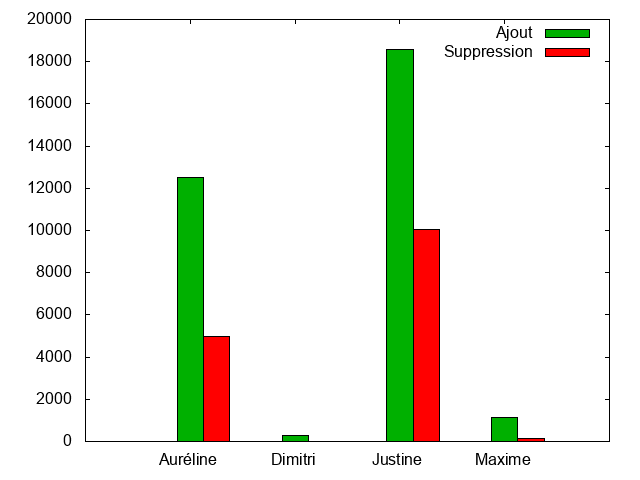
\includegraphics[width=0.66\textwidth, keepaspectratio]{img/repo_stats.png}
			\caption{Nombre de lignes ajoutés et supprimés par personne}
		\end{figure}

	\section{Idées d'améliorations}

		Notre application n'ayant pu être terminée faute de temps, voici la liste des améliorations que nous aurions voulu faire et celles qui seraient possibles d'implémenter ensuite :

		\begin{itemize}
			\item{Concevoir deux types de fichier, l'un pour l'éditeur et l'autre pour le jeu. Le jeu serait une version épurée de celui de l'éditeur et ne contiendrait pas la position des noeuds, par exemple}
			\item{Une mise à jour d'un noeud qui transformerait/transférerait correctement les différents liens (au lieu de les supprimer dans la plupart des cas)}
			\item{Vérifier que le livre est valide pour être joué}
			\item{Déclencher plus d'exception si le livre est incorrect à la lecture / écriture}
			\item{Pouvoir "parser" les compétences dans du texte}
			\item{Gérer les shops et les champs auto dans le jeu}
			\item{Afficher les personnages et items inutilisés}
			\item{Indiquer si l'estimation de la difficulté est à jour ou non}
			\item{Améliorer l'intelligence de la fourmi (pouvoir estimer si un item est plus important qu'un autre, meilleure gestion des combats, ...)}
			\item{Ajouter et supprimer des skills au fil du jeu}
			\item{Ajout de paramètres aux skills (plutôt que d'avoir un simple nom)}
			\item{Afficher les chemins gagnants}
			\item{Enlever ou ajouter une somme d'argent à un personnage se fait sur une monnaie précise (ex : -5 dollards, +15 euros, etc). De même pour les prérequis et l'édition du personnage principal.}
			\item{Ajout d'un "Langage" simple permettant de manier des conditions et variables pour des prérequis notamment}
			\item{Possibilité d'avoir des pnj qui pourraient nous suivre dans l'aventure pour combattre ou pour dévérouiller certains passages par exemple.}
		\end{itemize}

	\section{Bugs et problèmes connus}

		Certains problèmes sont connus, en voici une liste non exhaustive une fois de plus :

		\begin{itemize}
			\item{Tests incomplets sur le Jeu}
			\item{Le BookNodeCombat n'est pas du tout pratique à utiliser}
			\item{Le changement d'ID d'un personnage ou d'un item ne met pas à jour les différents élements du livre (noeuds, choix, ...)}
			\item{Le zoom ne se fait pas selon la position actuelle de la souris mais du point supérieur gauche du GraphPane}
		\end{itemize}
